\documentclass[a4paper]{article}
\usepackage[T1]{fontenc}
\usepackage[utf8]{inputenc}
\usepackage[italian]{babel}
\usepackage{amsthm}
\usepackage{amssymb}
\usepackage{mathtools}
\usepackage{enumerate}
\newcommand{\B}{\mathbf}
\usepackage{graphicx}
\usepackage{courier}
\swapnumbers

\title{Progetto Programmazione e Calcolo Scientifico 2024}
\author{Luca Agostino, Tommaso Basile, Andrea Cigna}

\begin{document}

\maketitle
\begin{abstract}
Il progetto si propone di sviluppare un software avanzato in linguaggio C++ per l'analisi e la segmentazione di fratture in strutture poligonali. L'obiettivo principale è quello di individuare le tracce di fratture presenti in una data geometria poligonale e suddividere le fratture in sottopoligoni distinti sulla base delle tracce trovate. Il sistema utilizzerà le strutture dati più appropriate in termini di memoria allocata ed efficienza computazionale. Una volta identificate tutte le tracce presenti, le fratture verranno utilizzate per segmentare la geometria originale in più sottopoligoni, permettendo un'analisi dettagliata e la possibilità di eseguire ulteriori studi su ciascun frammento. Questo progetto troverà applicazione in diversi campi, inclusi l'ingegneria civile, la geologia e la scienza dei materiali, offrendo uno strumento efficace per la valutazione delle strutture fratturate e il miglioramento della loro gestione e riparazione.
\end{abstract}

\tableofcontents

\section{Individuazione delle tracce}
Per determinare tutte le tracce che appartengono ad una frattura, ovvero le intersezioni che si generano con altri poligoni appartenente allo stesso set di dati, procederemo con l'individuazione dei piani che contengono le fratture in modo da ottenere ottenere la retta di intersezione. A questo punto, se la questa retta interseca entrambi i poligoni, verranno generati quattro punti e in base alla loro posizione spaziale sarà possibile capire se la traccia è passante o meno per ognuno dei poligoni analizzati. In tutti gli altri casi, la traccia non viene generata. Ripeteremo questo procedimento per ogni coppia di fratture sufficientemente vicine.
\subsection{Piano passante per una frattura}
Date $N$ fratture con $n_i$ vertici ciascuna, denominiamo con $\B{P}^{(i)}_j$ il vertice $j$ della frattura $i$. I range di valori sono, quindi, $i=0,\dots,N-1$ e $j=0,\dots,n_i-1$. Pertanto, per ogni frattura $i$, abbiamo una $n_i$-upla $(\B{P}^{(i)}_0,\dots,\B{P}^{(i)}_{n_i-1})$. Cerchiamo l'equazione cartesiana del piano $\pi$ contenente la frattura, dando per assunto che effettivamente i vertici forniti appartengono tutti ad uno stesso piano e che, quindi, corrispondano effettivamente a un poligono nello spazio tridimensionale. Per semplicità di notazione omettiamo nelle trattazioni successive l'apice $(i)$, sottointendendo che ci stiamo riferendo alla traccia $i$-esima. Vogliamo arrivare a una scrittura di $\pi$ del tipo $$ax+by+cz=d.$$
Se denotiamo con ${\B{A}\B{B}}=(x_B-x_A,y_B-y_A,z_B-z_A)$ il vettore congiungente $\B{A}$ a $\B{B}$, un generico punto $\B{P}\in\mathbb{R}^3$ appartiene al piano passante per i punti $\B{P}_0,\B{P}_1,\B{P}_2$ se vale che 
\begin{equation}\label{eq:piano1}
(\B{P}_0\B{P}_1\wedge \B{P}_0\B{P}_2)\cdot \B{P}_0\B{P}=0,
\end{equation} 
cioè il vettore che congiunge $\B{P}_0$ a $\B{P}$ deve essere ortogonale al vettore normale al piano (detto giacitura) $\B{P}_0\B{P}_1\wedge \B{P}_0\B{P}_2$. 
La \eqref{eq:piano1} equivale a porre nullo il determinante della matrice avente per righe le componenti dei $3$ vettori rispetto alla base canonica di $\mathbb{R}^3$: 
$$
\det\begin{pmatrix} x-x_0 & y-y_0 & z-z_0 \\ x_1-x_0 & y_1-y_0 & z_1-z_0 \\x_2-x_0 & y_2-y_0 & z_2-z_0 \end{pmatrix}=0.
$$
Sviluppando il determinante con la regola di Laplace rispetto alla prima riga otteniamo un'equazione del tipo 
\begin{equation}\label{eq:piano2}
a\left(x-x_0\right)+b\left(y-y_0\right)+c\left(z-z_0\right)=0,
\end{equation} 
dove 
\[
\begin{aligned}
& a=\operatorname{det}\left(\begin{array}{ll} y_1-y_0 & z_1-z_0 \\ y_2-y_0 & z_2-z_0 \end{array}\right), \\
& b=-\operatorname{det}\left(\begin{array}{ll}x_1-x_0& z_1-z_0 \\ x_2-x_0 & z_2-z_0 \end{array}\right),\\
& c=\operatorname{det}\left(\begin{array}{ll} x_1-x_0 & y_1-y_0 \\ x_2-x_0 & y_2-y_0 \end{array}\right). 
\end{aligned}
\]
Esplicitiamo i prodotti a primo membro dell'equazione \eqref{eq:piano2} 
\[
\begin{aligned}
& a\left(x-x_0\right)+b\left(y-y_0\right)+c\left(z-z_0\right)=0, \\
& a x-a x_0+b y-b y_0+c z-c z_0=0, \\
& a x+b y+c z-a x_0-b y_0-c z_0=0.
\end{aligned}
\]
Chiamiamo
$$
d=-a x_0-b y_0-c z_0.
$$ 
Così facendo abbiamo ricavato l'equazione cartesiana del piano cercato 
$$
ax+by+cz=d,
$$ 
con $a,b,c$ non tutti nulli, non essendo tutti e tre i punti allineati.

\subsection{Retta di intersezione tra piani}
Date due fratture diverei $i$ e $j$, grazie a quanto detto sopra, riusciamo a trovare l'equazione cartesiana dei due piani contententi le fratture. Nel caso in cui i due piani non siano paralleli, ci proponiamo di ricavare l'equazione in forma parametrica della retta $r$ che si genera dall'intersezione dei due piani; siamo, cioè, in cerca di una scrittura del tipo $$\B{OP}=\B{OQ}+t\B{v},$$ con $t$ parametro reale e $\B{v}$ la direzione della retta. Scriviamo in un sistema le equazioni per i due piani in questo modo: 
$$
\begin{cases}
a_1x+b_1y+c_1z=d_1\\ 
a_2x+b_2y+c_2z=d_2
\end{cases}
$$ 
dove i pedici indicano il piano rappresentato. Per i due piani definiamo con 
$$
\B{n}_1=\B{P}_0\B{P}_1\wedge \B{P}_0\B{P}_2,\quad \B{n}_2 = \B{P}'_0\B{P}'_1\wedge \B{P}'_0\B{P}'_2
$$ 
le due giaciture. La direzione individuata dalla retta di intersezione è data dal vettore normale a entrambe le giaciture dei piani: 
$$
\B{v}=\B{n}_1\wedge \B{n}_2.
$$ 
Al fine di trovare $\B{Q}$, se $c_1\neq 0$ oppure $c_2\neq0$, battezziamo $z$ come parametro libero e, ponendolo pari a $0$, risolviamo il sistema lineare 
$$
\begin{cases}
a_1x+b_1y=d_1\\ 
a_2x+b_2y=d_2
\end{cases}
$$ 
trovando $\B{OQ}=(\overline{x},\overline{y},0)$. Allora la retta di intersezione $r$ è data in forma parametrica da 
$$
\begin{cases}
x=\overline{x}+tv_x \\ 
y=\overline{y}+tv_y \\ 
z=tv_z.
\end{cases}
$$

Se la retta di intersezione tra i due piani è parallela al piano $xy$, scegliamo un altro parametro libero (ad esempio $x$): il nostro obbiettivo è solamente avere un punto di partenza per essa.
\subsection{Punti di intersezione}
Per ogni coppia di vertici consecutivi $\B{P}_j,\B{P}_{j+1}$ scriviamo la retta passante per entrambi $r_j$ attraverso l'ascissa curvilinea $s$ in questo modo: 
$$
\B{OP}=\B{OP}_j+s\B{P}_j\B{P}_{j+1},
$$
pertanto solo per valori di $s$ in $(0,1)$ otteniamo un punto del lato della frattura. 
Consideriamo adesso due fratture, attraverso i punti $1$ e $2$ troviamo i piani che li contengono e la retta di intersezione (se esiste) tra le due.

Per ogni coppia di vertici consecutivi della prima frattura intersechiamo la retta $r$ di intersezione e la retta $r_j$:
$$
\begin{cases}
\B{OP}=\B{OQ}+t\B{v} \\ 
\B{OP}=\B{OP}j+s\B{P}_j\B{P}_{j+1}
\end{cases}
$$
per cui abbiamo $$\B{OQ}+t\B{v}=\B{OP}_j+s\B{P}_j\B{P}_{j+1},$$ ossia un sistema di $3$ equazioni nelle incognite $t,s$. Riscriviamolo in tal modo:
\begin{equation} \label{sis:parametri}
\begin{cases}
v_xt-(x_{j+1}-x_j)s=x_j-\overline{x} \\
v_yt-(y_{j+1}-y_j)s=y_j-\overline{y} \\
v_zt-(z_{j+1}-z_j)s=z_j-\overline{z} \\
\end{cases}
\end{equation}
Potrebbe succedere che il sistema non ammetta soluzioni, in tal caso le due rette non si intersecano, cioè la traccia non attraversa il lato $\B{P}j\B{P}{j+1}$. Altrimenti, in caso di sistema determinato otterremo la coppia $(s,t)$. Se $s\in[0,1]$ otteniamo effettivamente che il punto di intersezione giace sul lato $\B{P}j\B{P}{j+1}$ della prima frattura. Iteriamo il processo per tutti gli $n_i$ vertici della frattura e troveremo due punti $\B{Q}_1$ e $\B{Q}_2$, trovati attraverso l'intersezione tra $r$ e due lati distinti della frattura.

Alla stessa maniera, effettuiamo questi calcoli per la seconda frattura, trovando o intersezione nulla per ogni lato o due altri due punti $\B{Q}_3$ e $\B{Q}_4$.

Nel caso in cui troviamo i 4 punti di intersezione, associamo ad ognuno il valore di $t$ corrispondente trovato nel sistema \eqref{sis:parametri} e costruiamo due intervalli dell'asse reale ordinando i valori dei parametri: otteniamo allora $(a,b)$ e $(c,d)$, dove $a,b\in\{t_1,t_2\}$ e $c,d\in\{t_3,t_4\}$. Se poniamo $a=\text{min}\{t_1,t_2\}$, $b=\text{max}\{t_1,t_2\}$, $c=\text{min}\{t_3,t_4\}$ e $d=\text{max}\{t_3,t_4\}$, attraverso una funzione che calcoli l'intersezione tra questi due intervalli, verifichiamo che
\begin{enumerate} [(i)]
\item se $(a,b)\cap(c,d)=(a,c)$, allora si tratta di una traccia non passante e i suoi vertici sono $\B{Q}_1$ e $\B{Q}_3$;
\item se $(a,b)\cap(c,d)=(a,b)$, allora si tratta di una traccia passante per il poligono $1$ e i suoi vertici sono $\B{Q}_1$ e $\B{Q}_2$;
\item se $(a,b)\cap(c,d)=(b,d)$, allora si tratta di una traccia non passante e i suoi vertici sono $\B{Q}_2$ e $\B{Q}_4$;
\item se $(a,b)\cap(c,d)=(c,d)$, allora si tratta di una traccia passante per il poligono $2$ e i suoi vertici sono $\B{Q}_3$ e $\B{Q}_4$.
\end{enumerate}
Attraverso questo algoritmo abbiamo trovato i vertici delle tracce, il loro valore di \textbf{Tips} e anche le intersezioni dei prolungamenti di esse sui poligoni, il che risulterà molto utile in seguito.

\section{Determinazione dei sotto-poligoni generati per ogni frattura}

L'idea alla base della determinazione dei sotto-poligoni è la seguente: analizzando una frattura alla volta, esaminiamo tutte le tracce per ordine di lunghezza e valore di $\B{Tips}$ e dividiamo il poligono in cui si trova la traccia in due sotto-poligoni. Il procedimento si ferma non appena la traccia non è più passante per il sotto-poligono che stiamo analizzando, in questo caso dividiamo un'ultima volta il poligono e passeremo alla traccia successiva. 

L'approccio che abbiamo utilizzato per implementare la determinazione dei sotto-poligoni è iterativo e può essere sintetizzato come segue.  

\subsection{Individuazione del punto iniziale}

Per ogni frattura dovremo creare una cella 2D iniziale che rappresenti il poligono di partenza, quindi verranno memorizzati tutti i vertici e i lati della frattura. Ad ogni vertice corrispondono le rispettive coordinate, mentre ad ogni lato sono assegnati gli identificativi dei vertici che lo generano. \\

Per ogni frattura $j=1,\dots,N$, consideriamo, una per volta, le tracce che le appartengono. Queste avranno una coppia di vertici $(\B T_{1},\B T_{2})$, quindi selezioniamo la cella 1D più vicina al punto $\B T_1$ attraverso i valori dell'ascissa curvilinea $s$ più prossimi a $0$; tale cella verrà selezionata all'interno della struttura attualmente presente, individuata dalla coppia $(\B P_{j},\B P_{j+1})$. Il punto situato alla sinistra di $\B T_1$ così individuato sarà il punto iniziale della suddivisione dei sotto-poligoni. Consideriamo il sistema

\begin{equation}
\begin{cases}
\B{OP}=\B{OT}_1+s\B{T}_1\B{T}_{2} \\ 
\B{OP}=\B{OP}_j+t\B{P}_j\B{P}_{j+1}
\end{cases}
\label{eq:intersezioni}
\end{equation}

Risolviamolo per determinare l'intersezione tra la traccia e ogni lato. Per cui abbiamo $$\B{OT}_{1}+s\B{T}_{1}\B T_{2}=\B{OP}_j+t\B{P}_j\B{P}_{j+1},$$ ossia un sistema di $3$ equazioni nelle incognite $t,s$. Riscriviamolo in tal modo:
\begin{equation} \label{sis:parametri}
\begin{cases}
(\tilde{x}_{2}-\tilde{x}_1)s-(x_{j+1}-x_j)t=x_j-\tilde{x}_1 \\
(\tilde{y}_{2}-\tilde{y}_1)s-(y_{j+1}-y_j)t=y_j-\tilde{y}_1 \\
(\tilde{z}_{2}-\tilde{z}_1)s-(z_{j+1}-z_j)t=z_j-\tilde{z}_1 \\
\end{cases}
\end{equation}

Potrebbe succedere che il sistema non abbia soluzione, in tal caso le rette sono parallele. Altrimenti in caso di sistema determinato otterremo la coppia $( s,t )$. Se $t \in [0,1]$ otteniamo effettivamente che il punto di intersezione giace sul lato $\B{P}_{j}\B{P}_{j+1}$, inoltre se $s \in [0,1]$ allora il punto si troverà sulla traccia stessa. Se, invece, $s$ non è mai compreso nell'intervallo $[0,1]$, significa che la traccia è interamente contenuta nella cella 2D. Ripetiamo tale procedura per tutte le celle 1D relative alla frattura di riferimento e scegliamo di volta in volta il valore di $s$ più vicino a 0 (nel caso in cui sia effettivamente uguale a $0$ avremo che il punto iniziale della traccia giace su un lato).
Quindi, memorizziamo in \texttt{idPreviousPoint} e in \texttt{idSuccessivePoint} i vertici del lato di partenza che è relativo al valore di $s$ più vicno a $0$, in \texttt{idIntersectionEdge} l'identificativo del lato $\B{P}_{j}\B{P}_{j+1}$ trovato, così come in \texttt{idIntersectionPoint} il punto di intersezione stesso individuato attraverso la risoluzione del sistema sopra citato. 

Adesso dividiamo la cella 1D che contiene il punto di intersezione in due nuove celle 1D, queste verranno memorizzate con codice identificativo e vertici nella struttura \texttt{PolygonalMesh}. Inoltre, ad ogni cella 1D creata verranno assegnati: 
\begin{enumerate} 
\item un booleano \texttt{isOn1D} per indicare se è attivo ($true$), cioè fa parte della struttura corrente, oppure se non lo è ($false$);
\item i codici identificativi delle fratture adiacenti al lato, al massimo due.
\end{enumerate}

Quindi la cella 1D appena divisa assumerà il booleano $false$ poiché esce dalla struttura corrente, mentre le due nuove celle 1D create acquisiscono l'attivazione e l'adiacenza alla cella 2D che stiamo analizzando. Anche per le celle 2D, che saranno sottoposte a suddivisioni, associamo un booleano \texttt{isOn2D}, per stabilire se la cella 2D appartenga ancora o no alla mesh.

\subsection{Creazione dei sotto-poligoni}
Prima di procedere con la suddivisione del poligono, dovremo fare attenzione a due casi: 
\begin{enumerate} [(i)]
\item se la traccia è interamente contenuta nel poligono allora dovremo suddividerlo in due sotto-poligoni (aggiornando le celle 2D adiacenti al lato di intersezione) e passare alla traccia successiva;
\item se la traccia continua su un altro poligono al di fuori di quello che stiamo analizzando, dovremo ripetere l'operazione di suddivisione anche per il poligono successivo, il cui identificativo si trova nel dato dei vicini al lato di intersezione.
\end{enumerate}

Per creare due nuove celle 2D, che rappresenteranno i due sotto-poligoni, è necessario assegnare alle celle i rispettivi lati creati, attivarli attraverso il booleano \texttt{isOn1D} e spegnere il poligono da cui provengono ponendo il campo \texttt{isOn2D} della cella al valore \emph{false}.

Partendo dal vertice \texttt{idSuccessivePoint}, e spostandoci in senso antiorario sul poligono da suddividere, assegneremo vertici e lati ai sotto-poligoni in base alla seguente casistica.
Un lato e un vertice saranno inseriti: 
\begin{enumerate} 
\item nel primo sotto-poligono, se il punto di intersezione con la retta della traccia non è ancora stato raggiunto;
\item nel secondo sotto-poligono, se il punto di intersezione con la retta della traccia è già stato superato.
\end{enumerate}
Per verificare la condizione di intersezione ripetiamo, per tutti i lati, il sistema \eqref{eq:intersezioni}. Quindi, se esiste l'intersezione e il parametro $t \in [0,1]$, allora il secondo estremo della traccia sta sul lato considerato che verrà diviso e disattivato, inoltre verrano memorizzati: 
\begin{itemize} 
\item \texttt{idNewIntersectionPoint} il secondo punto di suddivisione del poligono;
\item \texttt{idNewPreviousPoint} il punto finale del lato contenente l'intersezione;
\item \texttt{idNewSuccessivePoint} il punto di partenza del lato contenente l'intersezione;
\end{itemize}
Dopo aver creato i due sotto-lati ed averli memorizzati correttamente, è possibile continuare l'assegnazione dei lati del poligono originale nel secondo sotto-poligono. Il passaggio da un poligono all'altro può essere segnalato da un booleano che si attiva non appena troviamo l'intersezione. Per ultimo aggiungiamo ad entrambi i sotto-poligoni il lato che li divide con l'accortezza di assegnare, come vicini a questo lato, le due nuove celle create.
A questo punto, se la traccia iniziale non era interamente contenuta nel poligono, vengono assegnati:
\begin{itemize} 
\item \texttt{idIntersectionPoint} a \texttt{idNewIntersectionPoint};
\item \texttt{idPreviousPoint} a \texttt{idNewPreviousPoint};
\item \texttt{idSuccessivePoint} a \texttt{idNewSuccessivePoint};
\end{itemize}
in modo tale che il nuovo punto di partenza per la suddivisione del poligono adiacente sia il secondo punto di intersezione della prima suddivisione.

Questo procedimento viene iterato per ogni traccia del poligono originale finché il punto di intersezione della traccia con i lati del poligono, ottenuto mediante il sistema \eqref{eq:intersezioni}, ha l'ascissa curvilinea $s \in [0,1]$. Non appena troveremo un valore al di fuori di questo intervallo, concluderemo la divisione del poligono in cui è presente la traccia, aggiorneremo il poligono adiacente e passeremo alla traccia successiva, fino ad esaurirle completamente.

L'aggiornamento del poligono adiacente va fatto solo nel caso in cui questo esista, e consiste nella sostituzione dell'unico lato che risulterà spento, ovvero il lato adiacente, con i due nuovi sotto-lati generati dall'ultima suddivisione e con l'aggiunta dell'ultimo punto di intersezione.




\subsection{Esempio}
Di seguito considereremo un esempio chiarificatore. Le notazioni fin qui adottate saranno semplificate ulteriormente al fine di favorire al meglio l'esposizione. Consideriamo una sola frattura (Figura \ref{fig:esempio}) identificata da 4 vertici: $\B A$, $\B B$, $\B C$, $\B D$. 

\begin{figure}[h]
    \centering
    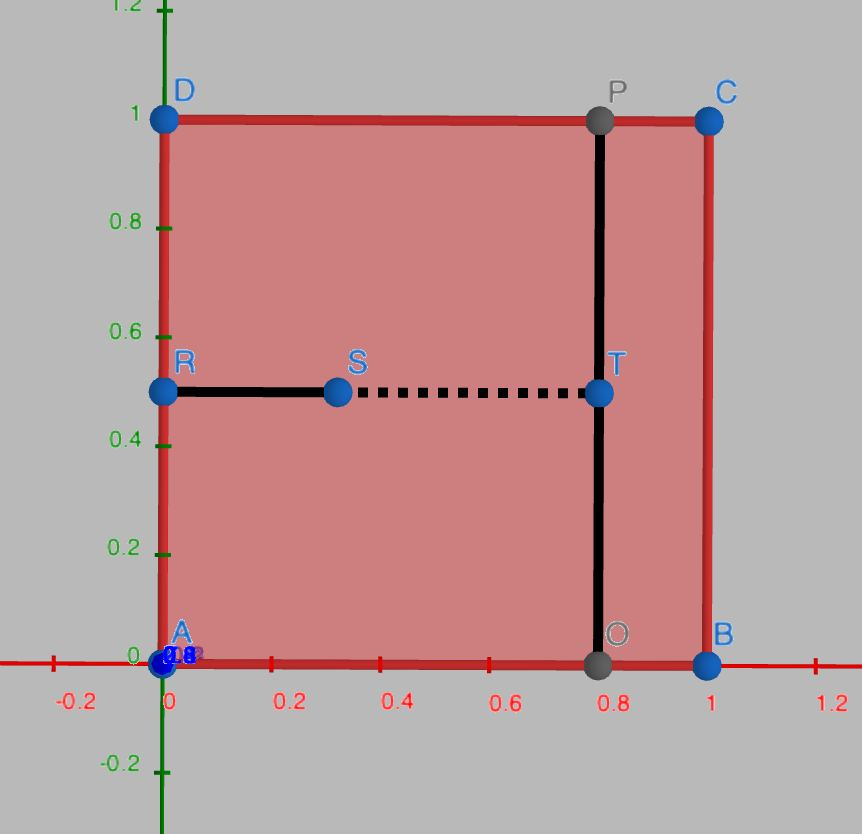
\includegraphics[width=11.5 cm]{im1.jpeg}
    \caption{Esempio}
    \label{fig:esempio}
\end{figure}

Su questa frattura consideriamo due tracce: la più lunga $\B{OP}$ e la più corta $\B{RS}$. Una volta trasferite le informazioni della frattura nella struttura \texttt{PolygonalMesh}, partiamo per ordine di lunghezza e scegliamo la traccia $\B{OP}$. Per ogni lato di $\B{ABCD}$, intersechiamo, usando il sistema \eqref{eq:intersezioni}, la traccia con esso: questo sistema avrà una soluzione con $t\in[0,1]$ solo per i lati $\B{AB}$ e $\B{CD}$. Scegliamo come \texttt{idIntersectionEdge} l'identificativo di $\B{AB}$ e aggiungiamo alla mesh il punto $\B O$ con un nuovo identificativo (sarà 4, in quanto i primi 4 vertici avranno rispettivamente 0,1,2,3).
 \texttt{idPreviousPoint}, \texttt{idIntersectionPoint} e \texttt{idSuccessivePoint} saranno, rispettivamente, 0, l'identificativo di $\B A$, 4 e 1, l'id di $\B B$. Procediamo allo spegnimento di $\B{AB}$ e inseriamo nella struttura le nuove sotto-celle 1D $\B{AO}$ e $\B{OB}$, attivandole e inserendo nella struttura di adiacenza gli identificativi dei due nuovi sotto-poligoni che andremo a costruire (saranno quelli di $\B{OBCP}$ e $\B{OPDA}$). Prima di operare le intersezioni con tutti i lati, provvediamo ad inserire al primo sotto-poligono che genereremo il lato $\B{OB}$. Ora, ciclando sui lati di $\B{ABCD}$ a partire da \texttt{idSuccessivePoint} (ossia $\B{B}$), intersechiamo la retta contenente la traccia con ognuno di essi: \begin{itemize} \item i vertici $\B{B}$, $\B C$ e il lato $\B{BC}$ apparterrano al primo sottopoligono che genereremo attraverso il taglio. Aggiorniamo, come sempre, anche la struttura di adiacenza; \item il lato $\B{CD}$ genererà una cella 0D (il punto $\B{P}$) e altre due sotto-celle 1D, alla stessa maniera di $\B{AB}$: perciò dovremo procedere all'inserimento del vertice $\B C$ nel primo sotto-poligono, allo spegnimento del lato $\B{CD}$, all'aggiornamento delle adiacenze dei due nuovi sotto-lati generati $\B{CP}$ e $\B{PD}$ e all'assegnazione di essi a $\B{OBCP}$ e $\B{OPDA}$. A questo punto, ogni lato che andremo ad aggiungere apparterrà al secondo sotto-poligono. \item Continuiamo l'inserimento di vertici e lati nel secondo sotto-poligono fino all'esaurimento dei lati, in questo caso fino al lato $\B{DA}$. \end{itemize} Ci resta da trattare il lato $\B{AB}$. Abbiamo già provveduto ad inserire $\B{OB}$ al primo sotto-poligono; ora possiamo inserire i vertici $\B A$, $\B O$ e il lato $\B{AO}$ al primo sotto-poligono. Provvediamo, infine, ad aggiungere il lato $\B{OP}$ ai due sotto-poligoni generati, aggiungendo ad esso le rispettive informazioni di adiacenza (i suoi vicini saranno entrambi i nuovi sotto-poligoni). Possiamo adesso procedere allo spegnimento del booleano relativo alla presenza della cella 2D $\B{ABCD}$, poichè è stata suddivisa e non più esistente.


Allo stesso modo, per la traccia $\B{RS}$, troveremo come punto iniziale il punto $\B{R}$ e procederemo identicamente. Dovremo avere l'accortezza di notare che il poligono da suddividere sarà $\B{OPDA}$ e che il poligono $\B{OBCP}$ dovrà essere modificato, in quanto gli verrà aggiunto il nuovo vertice $\B T$ e i nuovi lati $\B{PT}$ e $\B{TO}$.
\end{document}